
\chapter{Empirische Analyse bedinger Unabhängigkeit}
\label{ch:empirical-analysis}

Die vorangegangenen Abschnitte liefern für jede betrachtete Semantik eine
QBF-Kodierung der bedingten Unabhängigkeit. Im Folgenden wird beschrieben, wie diese
Kodierungen auf eine gemeinsame Auswahl an Benchmarkinstanzen angewendet und unter
kontrollierter Variation der Konditionierungsmenge empirisch untersucht
wurden. Eine Prüfkonfiguration besteht aus einem Argumentationssystem
\(F=(A,R)\), einer Semantik
\(\sigma\in\{\mathsf{st},\mathsf{co},\mathsf{pr}\}\), zwei
Singletonmengen \(X=\{x\}\) und \(Y=\{y\}\) sowie einer
Konditionierungsmenge \(Z\). Erfasst wurden der logische Solverstatus, die
für Übersetzung und Lösung benötigten Laufzeiten und Größenmerkmale der
erzeugten QBF.

\paragraph{Testinstanzen}
Die Ausgangsinstanzen stammen aus der AF-Kuration der sechsten
International Competition on Computational Models of Argumentation
(ICCMA'25) \cite{apostolakis:2025:iccma-instances}. Aus diesem Bestand
wurde vor Beginn des Experiments eine Auswahl aus sieben Familien
zusammengestellt. Sie umfasst drei klassische Zufallsgraphmodelle,
dedizierte AF-Generatoren sowie aus ABA- beziehungsweise Planungsinstanzen
erzeugte Argumentationssysteme. Tabelle~\ref{tab:experimental-instance-corpus}
zeigt die Zusammensetzung nach Anwendung des Größenfilters.

\begin{table}[htbp]
    \centering
    \begin{tabularx}{\textwidth}{@{}lXr@{}}
        \toprule
        Instanzfamilie & Struktur beziehungsweise Herkunft & Anzahl \\
        \midrule
        ABA2AF & aus ABA-Instanzen erzeugte AFs & 14 \\
        Barabási--Albert & skalenfreies Zufallsgraphmodell & 20 \\
        Erdős--Rényi & Zufallsgraphmodell mit unabhängigen Kanten & 20 \\
        Planning2AF & aus Planungsinstanzen erzeugte AFs & 5 \\
        SCC-Generator & AFs mit gezielt erzeugter SCC-Struktur & 6 \\
        Stable-Generator & mit einem dedizierten AF-Generator erzeugte Instanzen & 20 \\
        Watts--Strogatz & Small-World-Zufallsgraphmodell & 20 \\
        \midrule
        Insgesamt & & 105 \\
        \bottomrule
    \end{tabularx}
    \caption{Überblick über die Testinstanzen}
    \label{tab:experimental-instance-corpus}
\end{table}

Die Argumentanzahl \(n=|A|\) wurde jeweils aus der Kopfzeile
\texttt{p af N} der ICCMA-Datei gelesen. Berücksichtigt wurden sämtliche
vorab kuratierten Instanzen mit
\(
  100\leq n\leq 1\,000.
\)
Damit enthält das Untersuchungskorpus 105 AFs mit tatsächlich 100 bis
981 Argumenten. Die
Auswahl erfolgte weder anhand der späteren Solverstatus noch anhand der
gemessenen Laufzeiten. Verarbeitet wurden ausschließlich die bereitgestellten
\texttt{.af}-Dateien.

\paragraph{Konstruktion der Unabhängigkeitsanfrage}
\label{subsec:query-construction}

Für jedes Argumentationssystem \(F=(A,R)\) wurden zunächst fünf
verschiedene ungeordnete Paare \(\{x,y\}\subseteq A\) gleichverteilt und
ohne Wiederholung ausgewählt. Hieraus entstehen die Singletonmengen
\(X=\{x\}\) und \(Y=\{y\}\).

Die verwandte Pseudozufallsauswahl ist reproduzierbar. Der globale Ausgangswert ist
\texttt{SEED=42}. Für jede Instanz wird aus der Zeichenkette, die diesen
Wert und den Instanznamen enthält, ein instanzspezifischer
Seed abgeleitet. Daher untersuchen \emph{stable}, \emph{complete} und \emph{preferred}
dieselben fünf Argumentpaare.

Zu jedem Paar wurden sechs Größenstufen betrachtet. Für
\(\sigma\in\{\mathsf{st},\mathsf{co},\mathsf{pr}\}\) sei
\[
    d_\sigma=
    \begin{cases}
        5,  & \sigma\in\{\mathsf{st},\mathsf{co}\},\\
        10, & \sigma=\mathsf{pr},
    \end{cases}
    \qquad
    s_k^\sigma(n)=
    \left\lfloor
        \frac{k\lfloor n/d_\sigma\rfloor}{5}+\frac{1}{2}
    \right\rfloor,
    \quad k\in\{0,\ldots,5\}.
\]
Für jedes Paar, jede Semantik und jede Stufe wurde eine Menge
\(
    Z_{k,x,y}^{\sigma}\subseteq A\setminus\{x,y\},
    |Z_{k,x,y}^{\sigma}|=s_k^\sigma(n),
\)
gleichverteilt ohne Zurücklegen gezogen und anschließend numerisch
sortiert. Insbesondere ist \(Z_{0,x,y}^{\sigma}=\varnothing\). \emph{stable} und \emph{complete}
verwenden aufgrund derselben Größen und derselben Zufallsfolge identische
Konditionierungsmengen. \emph{preferred} verwendet dieselben Argumentpaare, aber
Stufen bis höchstens \(\lfloor n/10\rfloor\) und damit im Allgemeinen
andere Konditionierungsmengen. Die Maximalstufe beträgt bei \emph{stable} und
\emph{complete} \(\lfloor n/5\rfloor\).

Aus 105 Argumentationssystemen, fünf Paaren und sechs Größenstufen ergeben
sich je Semantik
\(
    105\cdot5\cdot6=3\,150
\)
Anfragen. Über alle drei Semantiken wurden somit \(9\,450\) QBF-Instanzen
erzeugt.

\paragraph{Erzeugung der QBF-Instanzen}
\label{subsec:qbf-generation}

Jede Instanz wurde mit der in
Theorem~\ref{thm:generic-independence-qbf-correct} beschriebenen Kodierung
in die geschlossene QBF
\(
    \Phi_F^\sigma(\{x\},\{y\}\mid Z_{k,x,y}^{\sigma})
\)
übersetzt. Die drei in Python implementierten Instanzgeneratoren und die
Anzahl ihrer quantifizierten Variablen sind in
Tabelle~\ref{tab:experimental-qbf-generators} zusammengefasst.

\begin{table}[htbp]
    \centering
    \begin{tabular}{@{}lll@{}}
        \toprule
        Semantik & Instanzgenerator & quantifizierte Variablen \\
        \midrule
        \emph{stable} & \texttt{af\_to\_stind\_qcir.py} & \(3n\) \\
        \emph{complete} & \texttt{af\_to\_coind\_qcir.py} & \(9n\) \\
        \emph{preferred} & \texttt{af\_to\_prind\_qcir.py} & \(18n\) \\
        \bottomrule
    \end{tabular}
    \caption{Semantikspezifische Generatoren der QBF-Instanzen.}
    \label{tab:experimental-qbf-generators}
\end{table}
Die Generatoren lesen das ICCMA-Format ein und bauen aus den
Angriffszeilen \texttt{i j} für jedes Argument die Menge seiner Angreifer
auf. Das Batchskript übergibt \(x\), \(y\) und die kommaseparierte Liste
der Elemente von \(Z\). Vor der Formelerzeugung wird geprüft,
ob alle Indizes im zulässigen Bereich liegen, innerhalb der drei Mengen
keine Duplikate auftreten und \(X\), \(Y\) und \(Z\) paarweise disjunkt
sind.

Die Generatoren schreiben alle quantifizierten Variablenblöcke und
Teilformeln unmittelbar im Format QCIR-G14. Eine Umwandlung in CNF oder
QDIMACS findet nicht statt. Die \emph{stable}-Kodierung verwendet boolesche
In-Mengen. \emph{complete} benötigt dreiwertige Labellings; \emph{preferred} ergänzt
Hilfslabellings für die Maximalitätsprüfung.

\paragraph{Solverausführung}
\label{subsec:solver-execution-protocol}

Das Batchskript \texttt{run\_batch\_singleton\_z.sh} führt die drei
Semantikphasen strikt in der Reihenfolge \emph{stable}, \emph{complete} und \emph{preferred}
aus. Eine Phase beginnt erst nach Abschluss der vorherigen. Innerhalb einer
Phase werden mehrere Argumentationssysteme parallel verarbeitet.

Die erzeugte QCIR-Datei wird ohne weitere Konvertierung an QuAbS
übergeben. Für jeden Solveraufruf gilt ein individuelles Zeitlimit von
\(600\,\mathrm{s}\), das ausschließlich die Solverausführung umfasst. Das
Batchskript setzt kein separates Speicherlimit. Jede vorgesehene Anfrage
wird genau einmal ausgeführt. Die Übersetzungs- und Solverlaufzeit werden
getrennt als Echtzeit gemessen. Nach erfolgreicher Übersetzung
werden außerdem die Anzahl der quantifizierten Variablen, die Zahl der
QCIR-Gatter und die Dateigröße in Byte bestimmt.

QuAbS signalisiert SAT regulär mit Rückgabecode 10 und UNSAT mit
Rückgabecode 20. Nach
Theorem~\ref{thm:generic-independence-qbf-correct} gilt damit
\(
    \text{SAT}
    \Longleftrightarrow
    \{x\}\perp_\sigma\{y\}\mid Z_{k,x,y}^{\sigma},
\)
während UNSAT die entsprechende Abhängigkeit bestätigt. Rückgabecode 124
des vorgeschalteten Zeitlimitprogramms wird als \texttt{TIMEOUT}
protokolliert. Bei anderen Rückgabecodes wird die Solverausgabe
noch auf eine eindeutige SAT- oder UNSAT-Zeile geprüft; ist auch dadurch
keine Entscheidung möglich, wird \texttt{SOLVER\_ERR} zusammen mit dem
Rückgabecode und der normalisierten Solvermeldung gespeichert. Nur SAT und
UNSAT werden als logische Ergebnisse interpretiert. Für alle übrigen
Status bleibt die Unabhängigkeitsaussage unbekannt.

Die semantikspezifischen CSV-Dateien enthalten 19 Spalten. Neben
Instanzname, \(n\), \(|R|\), Paarindex, \(x\), \(y\) und ihrer direkten
Angriffsbeziehung werden die Größenstufe, \(|Z|\) und die Elemente von
\(Z\) erfasst. Hinzu kommen Variablenzahl, Gatterzahl und Dateigröße der
QBF, beide Echtzeiten, Status, Rückgabecode, Solvermeldung und die
abgeleitete Kennzeichnung der Unabhängigkeit.

\emph{[Nach Abschluss des Reruns ergänzen: Prozessor,
Arbeitsspeicher, Betriebssystem, Python-, Bash- und QuAbS-Version sowie die
Zahl der parallelen AF-Worker.]}

\iffalse
\subsection{Versuchsdesign und Auswertungsmethode}
\label{subsec:empirical-stable-z-method}

Die Datengrundlage umfasst 107 Argumentationssysteme aus sieben
Instanzfamilien: ABA2AF, Barabási--Albert, Erdős--Rényi, Planning2AF,
SCC-Generator, Stable-Generator und Watts--Strogatz. Ausgewählt wurden AFs mit einer Argumentanzahl 
zwischen 100 und 1.000 aus 
den Instanzen der aktuellen ICCMA-Auswahl \cite{bistarelli:2025:iccma}.
Für jedes Argumentationssystem wurden fünf feste Argumentpaare \((x,y)\) untersucht.
Die Auswahl enthält 15 ABA2AF-Instanzen, jeweils 20
Barabási--Albert-, Erdős--Rényi-, Stable-Generator- und
Watts--Strogatz-Instanzen sowie jeweils sechs Planning2AF- und
SCC-Generator-Instanzen.
Jedes Paar wurde mit sechs Größenstufen der Konditionierungsmenge
ausgewertet. Insgesamt ergeben sich damit
\(107\cdot 5\cdot 6=3210\) Anfragen.

Für ein Argumentationssystem \(AF F =(A,R)\) mit \(n=|A|\) und einer Semantik \(\sigma \in \{st, co\}\) 
wurde die Größe der Stufe \(Z_k^{\sigma}\), \(k\in\{0,\ldots,5\}\), durch
\[
    |Z_k^{\sigma}|
    =
    \left\lfloor
        \frac{k\lfloor n/5\rfloor}{5}+\frac{1}{2}
    \right\rfloor
\]
bestimmt. Die Stufen entsprechen somit näherungsweise \(0\,\%\),
\(4\,\%\), \(8\,\%\), \(12\,\%\), \(16\,\%\) und \(20\,\%\) der Argumente.
Für jedes Paar und jede Stufe wurde genau
eine zu \(\{x,y\}\) disjunkte Menge \(Z_k\) mit festem Zufallsseed gezogen.
Die Mengen verschiedener Stufen wurden unabhängig voneinander gezogen.
Eine als SAT beendete QBF bestätigt nach
Theorem~\ref{thm:generic-independence-qbf-correct} die Relation
\(x\perp_{\mathsf{st}}y\mid Z\). UNSAT bestätigt entsprechend
\(x\not\perp_{\mathsf{st}}y\mid Z\). Die Ausgabe TIMEOUT erfolgt nach Erreichen des Zeitlimits von 600s. 
Anfragen, die bereits bei der Übersetzung nicht erzeugt werden können, werden als
Übersetzungsfehler separat ausgewiesen.

Die Ergebnisverteilung wird zunächst durch absolute Häufigkeiten und
Anteile beschrieben. Für die TIMEOUT-Rate werden nur tatsächlich gestartete
Solverläufe verwendet.
Der UNSAT-Anteil wird ausschließlich unter den gelösten Anfragen, also unter
SAT und UNSAT, berechnet. Zur Darstellung der Laufzeit wird für verschiedene
Zeitbudgets der Anteil aller 535 vorgesehenen Anfragen einer Stufe
angegeben, der innerhalb des Budgets gelöst wurde.

Zusätzlich werden die TIMEOUT-Anteile der Stufen \(Z_0\) und \(Z_5\)
miteinander verglichen. Hierzu wird für jedes Argumentationssystem und
jede der beiden Stufen der TIMEOUT-Anteil über die fünf untersuchten
Argumentpaare bestimmt. Die resultierenden gepaarten Werte werden mit
einem exakten zweiseitigen Vorzeichentest verglichen. Dabei gehen
Argumentationssysteme mit unverändertem TIMEOUT-Anteil nicht in die
Berechnung des \(p\)-Werts ein, werden jedoch separat berichtet.
\fi

\iffalse
\subsection{Ergebnisverteilung und Einfluss der Konditionierungsmenge}
\label{subsec:empirical-stable-z-status}

Tabelle~\ref{tab:empirical-stable-z-status} zeigt die beobachteten
Solverergebnisse. Die Zahl der TIMEOUTs steigt von 82 bei \(Z_0\) auf 113
bei \(Z_5\), während die Zahl der beobachteten UNSAT-Ergebnisse von 18 auf
2 zurückgeht. Die fünf Übersetzungsfehler treten ausschließlich in den drei
größten Stufen auf.

\begin{table}[tb]
    \centering
    \caption[Ergebnisse nach Größe der Konditionierungsmenge]{Ergebnisse der jeweils 535
    vorgesehenen Anfragen je \(Z\)-Stufe. Die TIMEOUT-Rate bezieht sich auf
    SAT, UNSAT und TIMEOUT; Übersetzungsfehler sind aus der Berechnung
    ausgeschlossen.}
    \label{tab:empirical-stable-z-status}
    \small
    \begin{tabular}{lrrrrrr}
        \toprule
        Stufe & SAT & UNSAT & TIMEOUT & Fehler
        & TIMEOUT-Rate \\
        \midrule
        \(Z_0\) & 435 & 18 & 82  & 0 & \(15{,}33\,\%\) \\
        \(Z_1\) & 441 & 10 & 84  & 0 & \(15{,}70\,\%\) \\
        \(Z_2\) & 436 & 7  & 92  & 0 & \(17{,}20\,\%\) \\
        \(Z_3\) & 436 & 3  & 95  & 1 & \(17{,}79\,\%\) \\
        \(Z_4\) & 430 & 2  & 101 & 2 & \(18{,}95\,\%\) \\
        \(Z_5\) & 418 & 2  & 113 & 2 & \(21{,}20\,\%\) \\
        \bottomrule
    \end{tabular}
\end{table}

\iffalse
Abbildung~\ref{fig:empirical-stable-z-composition} stellt dieselben
Häufigkeiten als Anteile dar. Der wachsende graue TIMEOUT-Anteil ist über
die Stufen hinweg deutlich erkennbar. Zugleich bleibt SAT in jeder Stufe
mit Abstand das häufigste beobachtete Ergebnis.


\begin{figure}[H]
    \centering
    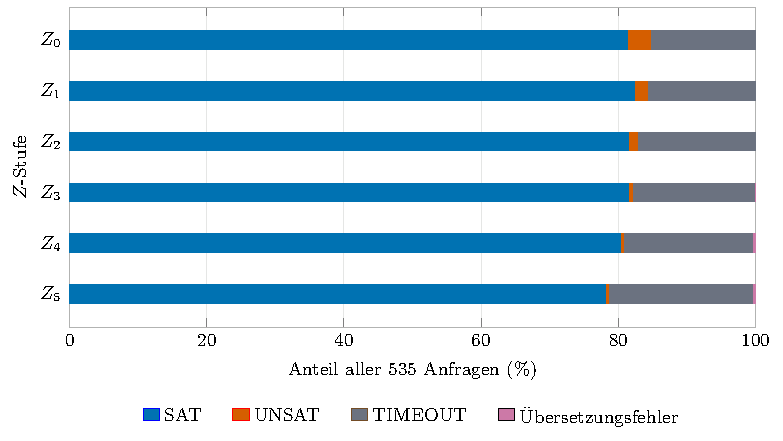
\includegraphics[width=\textwidth]
        {gfx/analysis_singleton_z_simple/statusverteilung.pdf}
    \caption[Ergebnisverteilung nach Größenstufe]{Relative
    Ergebnisverteilung der jeweils 535 vorgesehenen Anfragen. SAT
    bezeichnet nachgewiesene Unabhängigkeit, UNSAT nachgewiesene
    Abhängigkeit. TIMEOUTs und Übersetzungsfehler werden als eigene
    technische Kategorien ausgewiesen. Da hier der feste Nenner 535
    verwendet wird, unterscheiden sich die TIMEOUT-Anteile bei \(Z_3\) bis
    \(Z_5\) geringfügig von den um Übersetzungsfehler bereinigten Raten in
    Tabelle~\ref{tab:empirical-stable-z-status}.}
    \label{fig:empirical-stable-z-composition}
\end{figure}
\fi

Die bereinigte TIMEOUT-Rate nimmt von \(15{,}33\,\%\) bei \(Z_0\) auf
\(21{,}20\,\%\) bei \(Z_5\) zu. Dies entspricht einem Zuwachs von \(5{,}87\) Prozentpunkten. 
Die Rate steigt über alle sechs
Stufen hinweg schrittweise an. Demgegenüber sinkt der Anteil beobachteter
UNSAT-Ergebnisse unter den gelösten Anfragen von \(3{,}97\,\%\) auf
\(0{,}48\,\%\). Beide Verläufe sind in
Abbildung~\ref{fig:empirical-stable-z-rates} dargestellt.

\begin{figure}[H]
    \centering
    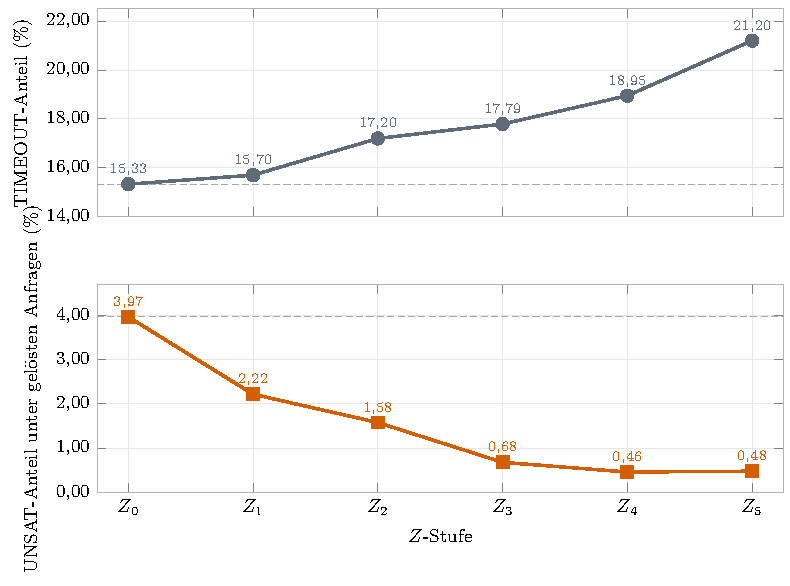
\includegraphics[width=\textwidth]
        {gfx/analysis_singleton_z_simple/ergebnistrends.pdf}
    \caption[Ergebnistrends nach Größenstufe]{TIMEOUT-Anteil unter den
    gültigen Solverläufen (oben) und UNSAT-Anteil unter den gelösten
    Anfragen (unten). Übersetzungsfehler sind aus der Berechnung
    ausgeschlossen. Die gestrichelte Linie markiert den Ausgangswert bei
    \(Z_0\).}
    \label{fig:empirical-stable-z-rates}
\end{figure}

Der Rückgang der beobachteten UNSAT-Ergebnisse darf nicht unmittelbar als
Rückgang der tatsächlichen Abhängigkeit interpretiert werden. Mit wachsendem
\(Z\) nimmt zugleich der Anteil der Anfragen zu, deren logischer Status
wegen eines TIMEOUTs unbekannt bleibt. Die Aussage beschränkt sich daher
darauf, dass unter den erfolgreich gelösten Anfragen seltener UNSAT
beobachtet wurde.

Für den Vorzeichentest können 105 Argumentationssysteme vollständig an
\(Z_0\) und \(Z_5\) verglichen werden. Zwei ABA2AF-Instanzen werden wegen
je eines Übersetzungsfehlers bei \(Z_5\) ausgeschlossen. Bei 95 der 105
Argumentationssysteme bleibt der TIMEOUT-Anteil unverändert. Zehn
Argumentationssysteme weisen bei \(Z_5\) einen höheren TIMEOUT-Anteil auf;
bei keinem nimmt er ab. Unter der Nullhypothese gleich wahrscheinlicher
Richtungen beträgt die Wahrscheinlichkeit für zehn gleichgerichtete
Änderungen im exakten zweiseitigen Vorzeichentest
\[
    p = 2\left(\frac{1}{2}\right)^{10}
      = 0{,}001953
      \approx 0{,}002.
\]
Bei einem vorab festgelegten Signifikanzniveau von
\(\alpha=0{,}05\) wird die Nullhypothese gleich wahrscheinlicher
Zu- und Abnahmen verworfen. Die Daten liefern damit Evidenz für einen
gerichteten Unterschied der beobachteten TIMEOUT-Anteile zwischen
\(Z_0\) und \(Z_5\).
Gleichzeitig zeigt
Abbildung~\ref{fig:empirical-stable-z-sign}, dass der Effekt nicht
gleichmäßig über alle Argumentationssysteme verteilt ist: Er konzentriert
sich auf zehn von 105 vollständig beobachteten Systemen
\((9{,}52\,\%)\), während der große Rest unverändert bleibt.

\begin{figure}[H]
    \centering
    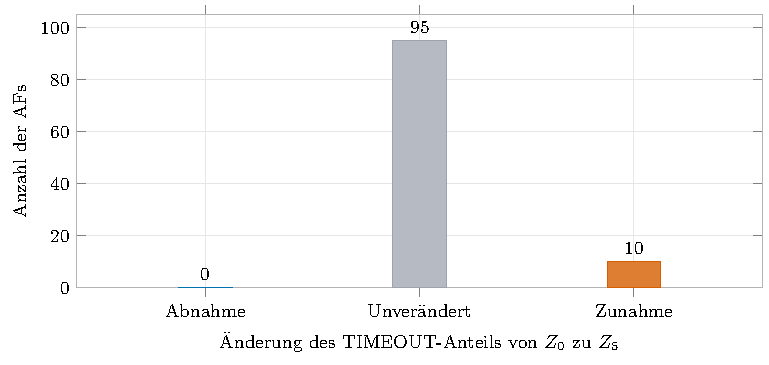
\includegraphics[width=\textwidth]
        {gfx/analysis_singleton_z_simple/vorzeichentest.pdf}
    \caption[AF-basierter Vergleich der kleinsten und größten Stufe]{Richtung der
    Änderung des TIMEOUT-Anteils zwischen \(Z_0\) und \(Z_5\) auf Ebene der
    Argumentationssysteme. Je System wurden die fünf Argumentpaare
    zusammengefasst. Dargestellt sind die 105 Systeme mit vollständig
    beobachteten Endpunkten. Zwei Systeme mit Übersetzungsfehler bei
    \(Z_5\) sind ausgeschlossen. Die 95 Bindungen werden berichtet, gehen
    aber nicht in den exakten Vorzeichentest ein.}
    \label{fig:empirical-stable-z-sign}
\end{figure}

\subsection{Unterschiede zwischen den Instanzfamilien}
\label{subsec:empirical-stable-z-families}

Die aggregierte Zunahme der TIMEOUT-Rate ist nicht für alle
Instanzfamilien gleichermaßen zu beobachten.
Abbildung~\ref{fig:empirical-stable-z-families} zeigt die TIMEOUT-Raten
getrennt nach Familie und \(Z\)-Stufe. Besonders deutlich ist der Effekt
für Barabási--Albert: Dort steigt die Rate von \(0\,\%\) bei \(Z_0\) auf
\(20\,\%\) bei \(Z_5\). Bei Planning2AF steigt sie bereits bis \(Z_2\) auf
\(33{,}3\,\%\) und bleibt anschließend auf diesem Niveau.

\begin{figure}[H]
    \centering
    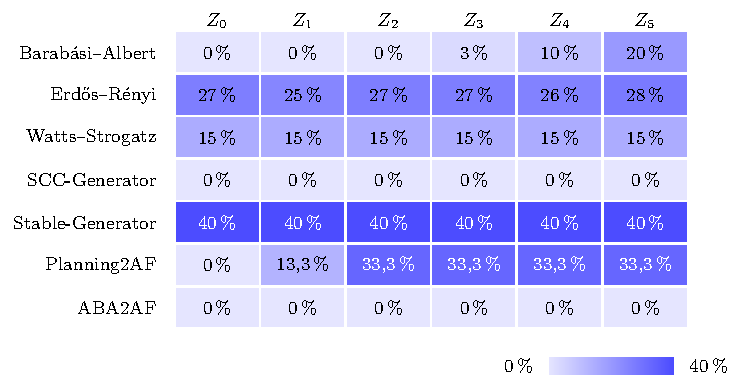
\includegraphics[width=\textwidth]
        {gfx/analysis_singleton_z_simple/familien-timeouts.pdf}
    \caption[TIMEOUT-Raten nach Instanzfamilie]{TIMEOUT-Rate in Prozent
    nach Instanzfamilie und \(Z\)-Stufe. Die Zellen sind auf eine
    Nachkommastelle gerundet. Übersetzungsfehler sind aus der Berechnung
    ausgeschlossen.}
    \label{fig:empirical-stable-z-families}
\end{figure}

Für Erdős--Rényi schwankt die Rate lediglich zwischen \(25\,\%\) und
\(28\,\%\). Beim Stable-Generator bleibt sie auf allen Stufen bei
\(40\,\%\), bei Watts--Strogatz bei \(15\,\%\). Für SCC-Generator und
ABA2AF treten keine TIMEOUTs auf. Von den zehn
Argumentationssystemen mit einer Zunahme im Endpunktvergleich stammen
sieben aus der Barabási--Albert-Familie, zwei aus Planning2AF und eines aus
Erdős--Rényi. Der allgemein beobachtete Trend lässt sich somit vor allem durch
Barabási--Albert und Planning2AF erklären. Eine allgemeine Aussage, nach
der ein größeres \(Z\) jedes Argumentationssystem erschwert, wäre somit aufgrund
der vorliegenden Daten nicht möglich.

\subsection{Solverlaufzeit}
\label{subsec:empirical-stable-z-runtime}

Neben der höheren TIMEOUT-Rate verschiebt sich auch der Anteil schnell
gelöster Anfragen. Abbildung~\ref{fig:empirical-stable-z-performance}
zeigt für jedes Zeitbudget \(t\), welcher Anteil aller 535 Anfragen einer
Stufe bis zu diesem Zeitpunkt gelöst wurde. Bei einem Budget von einer Sekunde
sinkt dieser Anteil von \(57{,}0\,\%\) bei \(Z_0\) auf \(45{,}2\,\%\) bei
\(Z_5\). Bei 100 Sekunden beträgt er \(81{,}3\,\%\) beziehungsweise
\(74{,}2\,\%\). Der Verlauf der Performanceprofile zeigt insgesamt: Mit
wachsendem \(Z\) wird ein kleinerer Anteil der Anfragen innerhalb desselben
Budgets gelöst.

\begin{figure}[H]
    \centering
    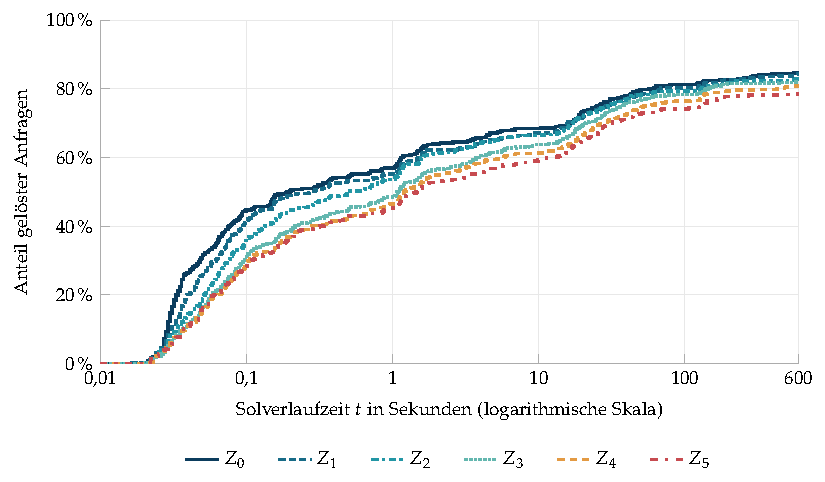
\includegraphics[width=\textwidth]
        {gfx/analysis_singleton_z_simple/performanceprofil.pdf}
    \caption[Performanceprofile nach Größe der Konditionierungsmenge]{Empirische
    Performanceprofile der sechs Größenstufen. Dargestellt ist für jedes
    Zeitbudget \(t\) der Anteil der je Stufe 535 vorgesehenen Anfragen, die
    bis \(t\) gelöst wurden. Die Zeitachse ist logarithmisch.}
    \label{fig:empirical-stable-z-performance}
\end{figure}

Dieser Unterschied lässt sich auch durch die Zeit bis zur Lösung der Hälfte
aller Anfragen ausdrücken. Bei \(Z_0\) sind \(50\,\%\) nach
\(0{,}198\) Sekunden gelöst, bei \(Z_5\) erst nach \(1{,}482\) Sekunden.
Das entspricht ungefähr dem Faktor \(7{,}5\).

\subsection{QBF-Größe und Erzeugungszeit}
\label{subsec:empirical-stable-z-qbf-overhead}

Die längeren Solverlaufzeiten können grundsätzlich zwei Ursachen haben. Zum
einen wächst mit \(Z\) die erzeugte QBF, sodass der Solver bereits rein
syntaktisch mehr Eingabedaten verarbeiten muss. Zum anderen verändert die
zusätzliche Konditionierung den logischen Aufbau der Formel und damit
möglicherweise die Schwierigkeit der internen Such- und
Propagationsschritte. Um beide Erklärungen deskriptiv gegenüberzustellen,
werden für jedes Argumentpaar die QBF-Kenngrößen einer Stufe mit den
Kenngrößen desselben Paars bei \(Z_0\) verglichen. Als Zusammenfassung wird
der Median der paarweisen Verhältnisse verwendet. Der Median ist für diesen
Vergleich geeignet, da einzelne ungewöhnlich lange Übersetzungs- oder
Solverläufe das Ergebnis weniger stark beeinflussen als bei einem
arithmetischen Mittel.

Für alle 3205 erfolgreich übersetzten Anfragen gelten exakt die Beziehungen
\[
    N_{\mathrm{var}} = 3n
    \qquad\text{und}\qquad
    N_{\mathrm{gate}} = 12n + 6|Z| + 16,
\]
wobei \(N_{\mathrm{var}}\) die Zahl der QBF-Variablen und
\(N_{\mathrm{gate}}\) die Zahl der QBF-Gatter bezeichnet. Die
Variablenzahl bleibt bei einer Änderung von \(Z\) folglich konstant. Jedes
zusätzliche Argument in \(Z\) fügt der verwendeten Kodierung dagegen genau
sechs Gatter hinzu.

\iffalse
Abbildung~\ref{fig:empirical-stable-z-qbf-overhead} zeigt, dass dieser
syntaktische Zuwachs über die Größenstufen annähernd linear verläuft. Bei
\(Z_5\) liegt die mediane Gatterzahl \(9{,}93\,\%\) und die mediane
QBF-Dateigröße \(6{,}53\,\%\) über dem jeweiligen Wert bei \(Z_0\). Die
mediane Übersetzungszeit nimmt demgegenüber lediglich um \(1{,}00\,\%\)
zu. Der größere Umfang der Kodierung verursacht somit nur einen geringen
zusätzlichen Aufwand bei der QBF-Erzeugung.

\begin{figure}[H]
    \centering
    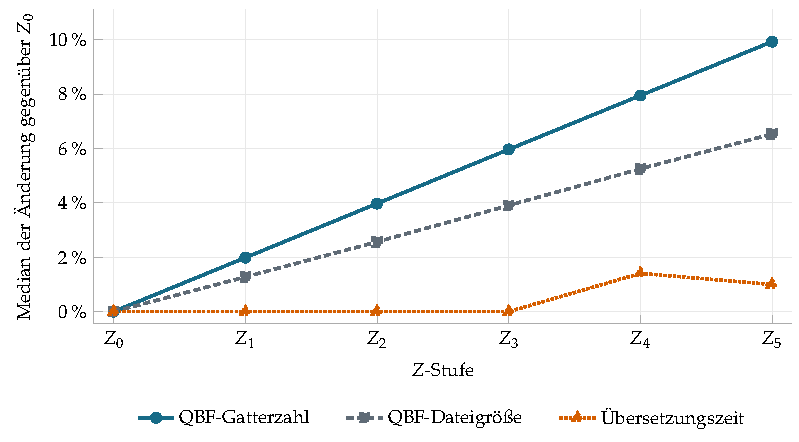
\includegraphics[width=\textwidth]
        {gfx/analysis_singleton_z_simple/qbf-overhead.pdf}
    \caption[QBF-Größe und Übersetzungszeit nach Größenstufe]{Median der
    paarweisen relativen Änderungen von QBF-Gatterzahl, QBF-Dateigröße und
    Übersetzungszeit gegenüber \(Z_0\). Verglichen wird jeweils dasselbe
    Argumentpaar; Paare mit einem Übersetzungsfehler am Vergleichsendpunkt
    werden ausgeschlossen. Es gehen 535 Paare bei \(Z_1\) und \(Z_2\), 534
    bei \(Z_3\) sowie 533 bei \(Z_4\) und \(Z_5\) ein. Die konstante
    QBF-Variablenzahl ist nicht dargestellt.}
    \label{fig:empirical-stable-z-qbf-overhead}
\end{figure}
\fi

Gegen eine ausschließlich durch die syntaktische Größe verursachte
Verlangsamung spricht insbesondere der Vergleich der Instanzfamilien in
Abbildung~\ref{fig:empirical-stable-z-qbf-runtime}. Die mediane
Gatterzahl steigt in jeder Familie von \(Z_0\) nach \(Z_5\) um ungefähr
den Faktor \(1{,}10\). Die mediane Solverlaufzeit erhöht sich bei
Barabási--Albert jedoch um den Faktor \(6{,}79\) und bei Planning2AF um
den Faktor \(5{,}04\). In den übrigen Familien liegt der Laufzeitfaktor
trotz eines nahezu identischen Gatterzuwachses nur zwischen \(1{,}00\)
und \(1{,}10\). Der Umfang der QBF allein ist daher keine hinreichende
Erklärung für die beobachtete Verlangsamung.

\begin{figure}[H]
    \centering
    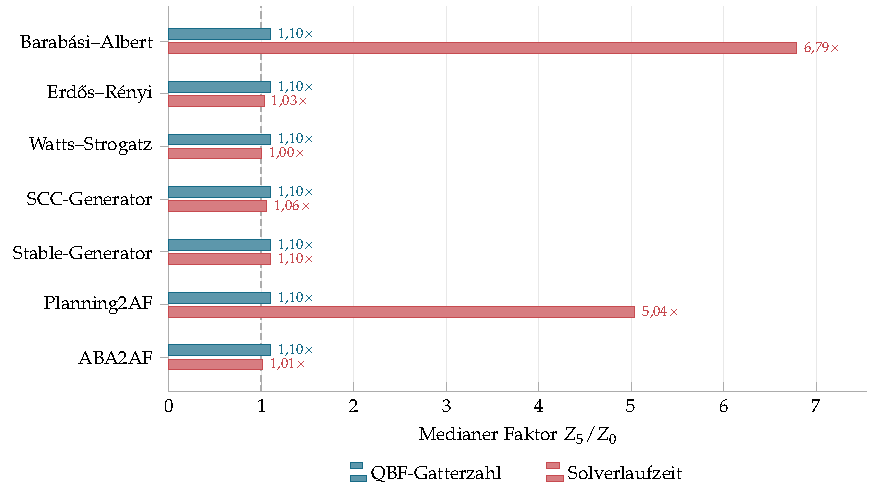
\includegraphics[width=\textwidth]
        {gfx/analysis_singleton_z_simple/qbf-runtime-vergleich.pdf}
    \caption[QBF-Größe und Solverlaufzeit nach Instanzfamilie]{Median der
    paarweisen Faktoren von \(Z_5\) gegenüber \(Z_0\), getrennt nach
    Instanzfamilie. Für die Gatterzahl werden Paare mit erfolgreicher
    Übersetzung an beiden Endpunkten berücksichtigt. Der Laufzeitfaktor
    umfasst nur Paare, die an beiden Endpunkten gelöst wurden. Die
    Laufzeitfaktoren beruhen in der dargestellten Reihenfolge auf 80, 71,
    85, 30, 60, 20 und 73 Paaren.}
    \label{fig:empirical-stable-z-qbf-runtime}
\end{figure}

Die Ergebnisse sprechen damit dafür, dass vor allem die durch ein größeres
\(Z\) veränderte logische Struktur die solverseitige Schwierigkeit erhöht,
während das moderate syntaktische Wachstum nur einen kleineren Anteil
erklärt. Eine eindeutige kausale Trennung ist mit dem vorliegenden
Versuchsaufbau jedoch nicht möglich, da eine größere Konditionierungsmenge 
gleichzeitig den Umfang und den logischen Inhalt der QBF verändert. 

\subsection{Einordnung und Einschränkungen}
\label{subsec:empirical-stable-z-limitations}

Die Auswertung zeigt im Durchschnitt einen klaren Zusammenhang zwischen einem
größeren \(Z\) und einer schwierigeren praktischen Lösung: für feste Zeitbudgets 
werden weniger Anfragen gelöst. Der
Vorzeichentest liefert zusätzliche Evidenz für die gerichtete Zunahme der
TIMEOUT-Rate zwischen \(Z_0\) und \(Z_5\). Die Auswertung der einzelnen Instanzfamilien
relativiert dieses Ergebnis jedoch: Die Erhöhung des TIMEOUT-Anteils im
Endpunktvergleich betrifft nur einen kleinen Teil der
Argumentationssysteme und wird hauptsächlich durch zwei Instanzfamilien
getragen.

Bei der Interpretation sind vier Einschränkungen wesentlich. Erstens sind
die Mengen \(Z_k\) unabhängig gezogen und nicht geschachtelt. Verglichen
werden daher zufällige Mengen unterschiedlicher Größe und nicht die
schrittweise Erweiterung einer festen Menge. Zweitens existiert je Paar
und Größenstufe nur eine Ziehung von \(Z_k\). Der Einfluss der Größe kann
somit nicht vollständig vom Einfluss der konkreten Zusammensetzung
getrennt werden. Drittens verdecken TIMEOUTs den logischen SAT- oder
UNSAT-Status. Insbesondere erlaubt der beobachtete Rückgang des
UNSAT-Anteils keine Aussage über den unbekannten Status der nicht gelösten
Anfragen. Viertens besteht die Datengrundlage aus einer Auswahl von
Benchmarkinstanzen. Eine uneingeschränkte Verallgemeinerung auf beliebige
andere Argumentationssysteme ist deshalb nicht gerechtfertigt.

Insgesamt stützen die Daten die Aussage, dass größere
Konditionierungsmengen die Lösung der Stable-QBFs im untersuchten
Benchmark erschweren können. Dieser Effekt ist in der Ergebnisverteilung
und in den Lösungsquoten sichtbar, fällt aber stark
familienabhängig aus und ist nicht bei jedem Argumentationssystem zu
beobachten. Der geringe Zuwachs von QBF-Größe und Übersetzungszeit reicht
als alleinige Erklärung für die ausgeprägten Laufzeiteffekte in den
Barabási--Albert- und Planning2AF-Instanzen nicht aus.
\fi

\section{Einfluss der Konditionierungsmenge auf den Unabhängigkeitsstatus}
\label{sec:Z-CI-influence}

\section{Einfluss der Konditionierungsmenge auf die Solverlaufzeit}
\label{sec:Z-runtime-influence}